\section{Zarządzanie projektem}

Ze względu na rozwojowy charakter projektu i~niedookreśloną formę produktu
końcowego do prowadzenia projektu starano się zaadaptować zwinną metodykę
\emph{Scrum}.
Jako długość sprintu przyjęto stały okres dwóch tygodni, po upłynięciu których,
począwszy od ostatniego tygodnia pierwszego semestru, sporządzany był zbiorowy
raport relacjonujący pracę wykonaną przez każdego członka zespołu.

W~początkowej fazie trwania projektu przed rozpoczęciem każdego sprintu
ustalane były zadania, które następnie podlegały estymacji przy użyciu techniki
o~nazwie \emph{Planning Poker}, w~której udział brali wszyscy członkowie
zespołu.
Ustalanie terminarza sprintów, zarządzanie zadaniami (w~tym przypisywanie
ich konkretnym osobom oraz śledzenie stanu wykonania), jak również
monitorowanie kondycji całego projektu możliwe było dzięki wykorzystaniu
serwisu \emph{Scrum'd}.

\begin{figure}[ht]
	\centering
		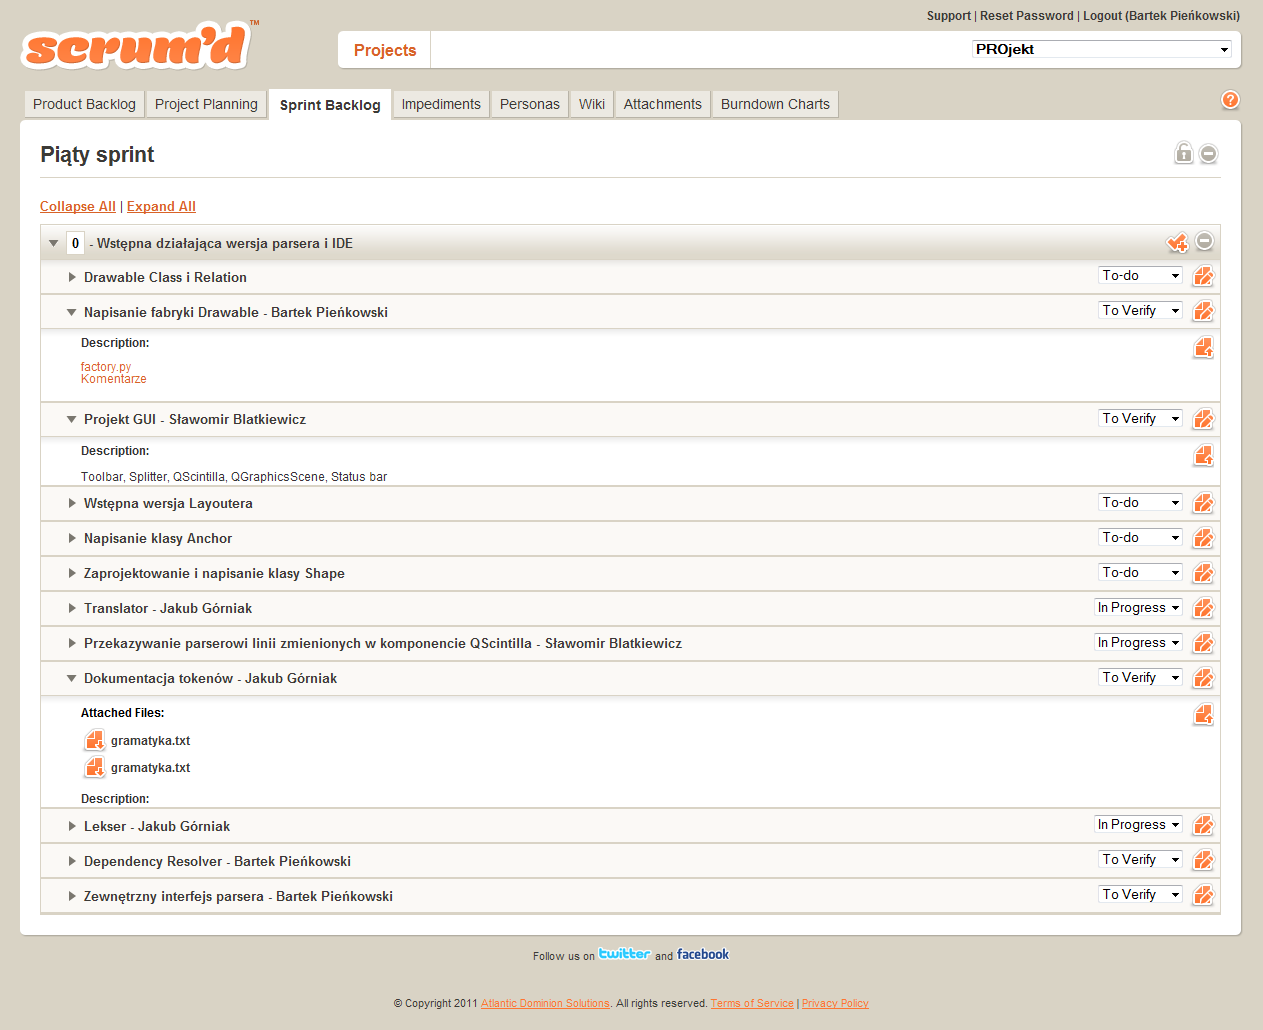
\includegraphics[scale=0.3]{scrumd}
	\caption{Wygląd listy zadań w~serwisie \emph{Scrum'd}}
	\label{fig:scrumd}
\end{figure}

Dążąc do zapewnienia wysokiej jakości tworzonego kodu każdy nowo powstały
fragment programu, przed dostaniem się do głównego repozytorium, weryfikowany
był przez kierownika projektu i~pozostałych członków zespołu w~celu wskazania
błędów i~odnotowania ewentualnych uwag. Komentowanie kodu z~dokładnością do
pojedynczej linii możliwe było dzięki bogatej funkcjonalności serwisu
\emph{GitHub}.

W~miarę upływu czasu każdy z~członków zespołu zaczął zajmować się określonym
obszarem projektu, dzięki czemu podział zadań stał się oczywisty. Podczas
wzmożonej pracy nad stworzeniem demonstracyjnej wersji programu większość zadań
przerodziła się w~drobne poprawki, czego efektem była (prawdopodobnie
niesłuszna) rezygnacja z~dalszej estymacji zadań.

W~celu przyspieszenia procesu integracji zorganizowano w~tamtym okresie kilka
spotkań w~laboratorium 225, na których stawiła się większość członków zespołu.
Zalety takiego sposobu pracy (szybkie tempo, ułatwiona komunikacja wewnątrz
zespołu) były niepodważalne. W~efekcie proces pełnej integracji kodu
zakończył się sukcesem.

Nowy sposób pracy narzucił wymóg korzystania z~bardziej odpowiedniego narzędzia
do zarządzania nim, zrezygnowano więc z~używania serwisu \emph{Scrum'd} na rzecz
o~wiele prostszego w~założeniach i~obsłudze serwisu \emph{Checkvist}, będącego
interaktywną listą zadań dającą możliwość współtworzenia wszystkim członkom
zespołu. Zakres możliwości tego narzędzia obejmuje dodawanie i~usuwanie zadań,
oznaczanie ich jako wykonanych, komentowanie oraz ustalanie terminarza.

\begin{figure}[ht]
	\centering
		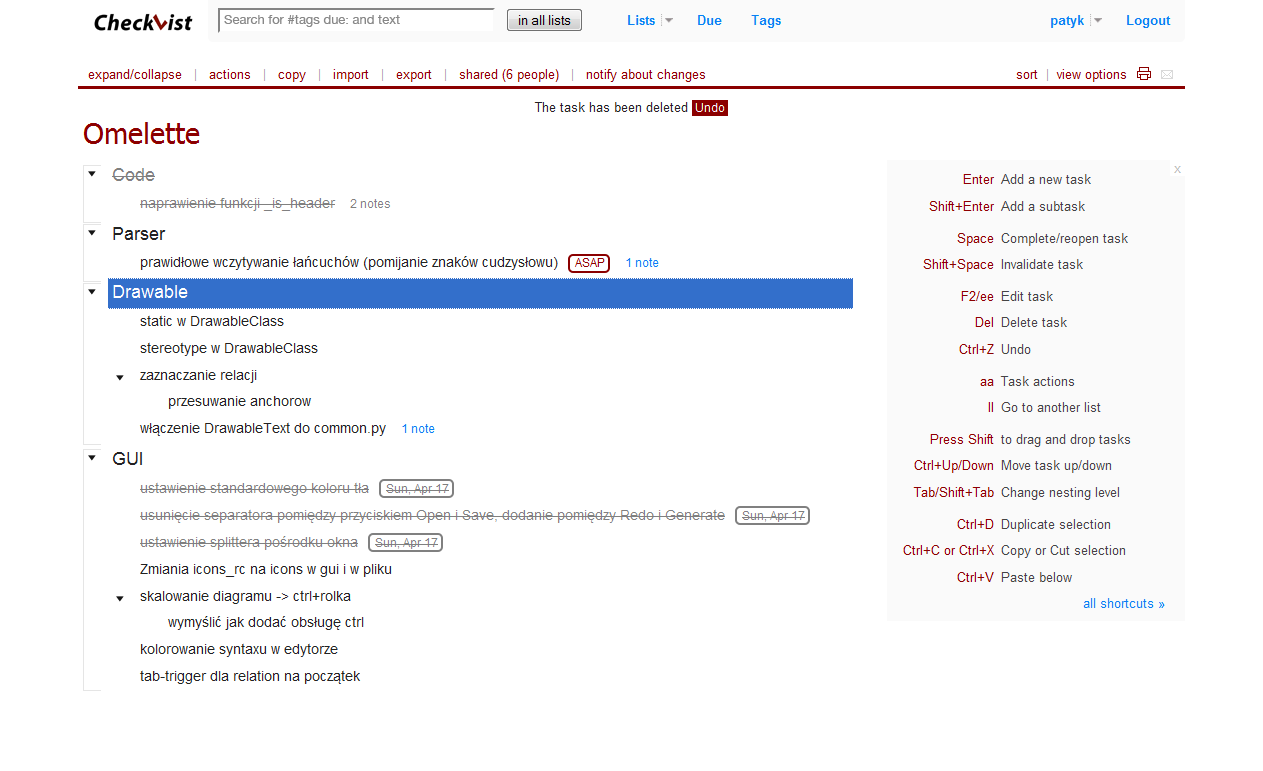
\includegraphics[scale=0.3]{checkvist}
	\caption{Wygląd listy zadań w~serwisie \emph{Checkvist}}
	\label{fig:checkvist}
\end{figure}

W~końcowej fazie projektu zaczęto wykorzystywać nowy \emph{issue tracker}
udostępniony w~ramach serwisu \emph{GitHub}. Zarządzanie zadaniami przy pomocy
tego narzędzia obejmowało m.in. przypisywanie ich konkretnym osobom, ustalanie
kamieni milowych i~dodawanie etykiet. Korzyścią wynikającą z~jego używania była
jawność zadań i~osób za nie odpowiedzialnych, jak również możliwość zamykania
wykonanych zadań udostępniona wszystkim członkom zespołu.

\begin{figure}[ht]
	\centering
		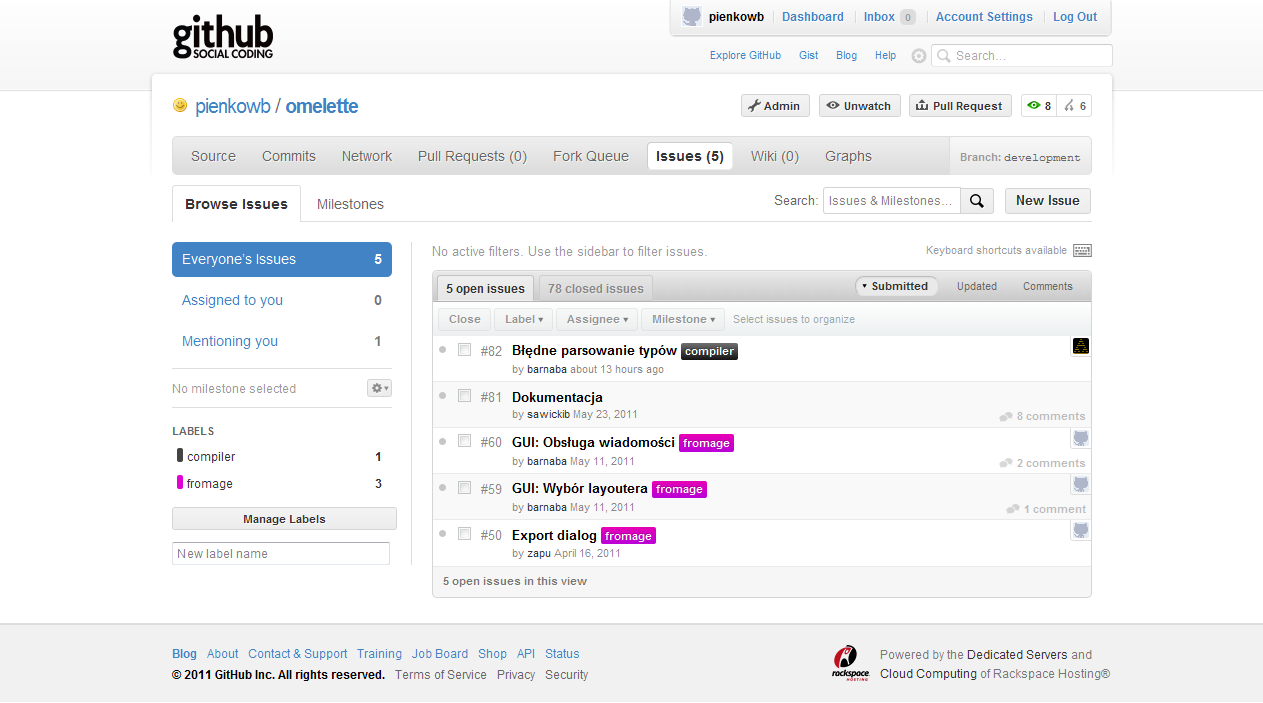
\includegraphics[scale=0.3]{github-issues}
	\caption{Nowy \emph{issue tracker} oferowany przez serwis \emph{GitHub}}
	\label{fig:github-issues}
\end{figure}

Oceniając projekt z~perspektywy kierownika można stwierdzić, iż niewątpliwą
trudnością w~zarządzaniu zespołem były opóźnienia w~dostarczaniu kodu przez
niektórych członków zespołu oraz problemy z~egzekwowaniem przydzielonych zadań.
Ostatecznie udało się w~dużym przybliżeniu zrealizować zamierzoną
funkcjonalność (która nie została przecież dokładnie sprecyzowana), więc
projekt nie okazał się porażką. Z~drugiej strony, mimo negatywnego nastawienia
niektórych członków zespołu, można było utrzymać bardziej wydajne tempo pracy.
